
%================
\chapter{MISUKE}
%================
本章では、MISUKEという概念について述べる。もともと本論文は研究室での日々とかを回顧録としてまとめた概念だと筆者の一人は思っていたが、なんか知らんけど書くことになった。
まあええか$\sf{ (´\_ゝ`)}$笑

%=================
\section{葱や平吉}
%=================
MISUKEの概念については次節で述べるとして、まずは葱や平吉である(図\ref{negiya})。
このお店は京都 河原町の繁華街から少し離れた小道沿いに存在する天ぷら料理屋である。中でも特徴的なのがネギで、なんか食べ放題とか。
\par
そもそもオガワマンとネギには切っても切れない(ネギなだけに)関係がある。
その一つは、オガワマンの同い年のいとこ(バラクスミス・ディエゴ・ホセ・クズバラ・フランシスコ・デ・パウラ・ファン・ネポムセーノ・マリア・デ・ロス・レメディオス・クリスピン・クリスピアーノ・デ・ラ・サンティシマ・トリニダード・ルイス・ネスコ・オバスミコス・ベースボールブラザーズ)\index{ばらくすみす@バラクスミス・ディエゴ・ホセ・クズバラ・フランシスコ・デ・パウラ・ファン・ネポムセーノ・マリア・デ・ロス・レメディオス・クリスピン・クリスピアーノ・デ・ラ・サンティシマ・トリニダード・ルイス・ネスコ・オバスミコス・ベースボールブラザーズ}である(図\ref{itoko})。
オガワマン\index{おがわまん@オガワマン}が幼稚園のころ、いとこがネギが嫌いと言いだして、事あるごとにネギを避けていたため、オガワマン\index{おがわまん@オガワマン}もなぜか嫌いになったという過去がある。小学生になっていとこと会う回数が減ってからはいつの間にかネギ嫌いではなくなっており、今はむしろ好きである。バラッッッッッッ

\begin{figure}[H]
\centering
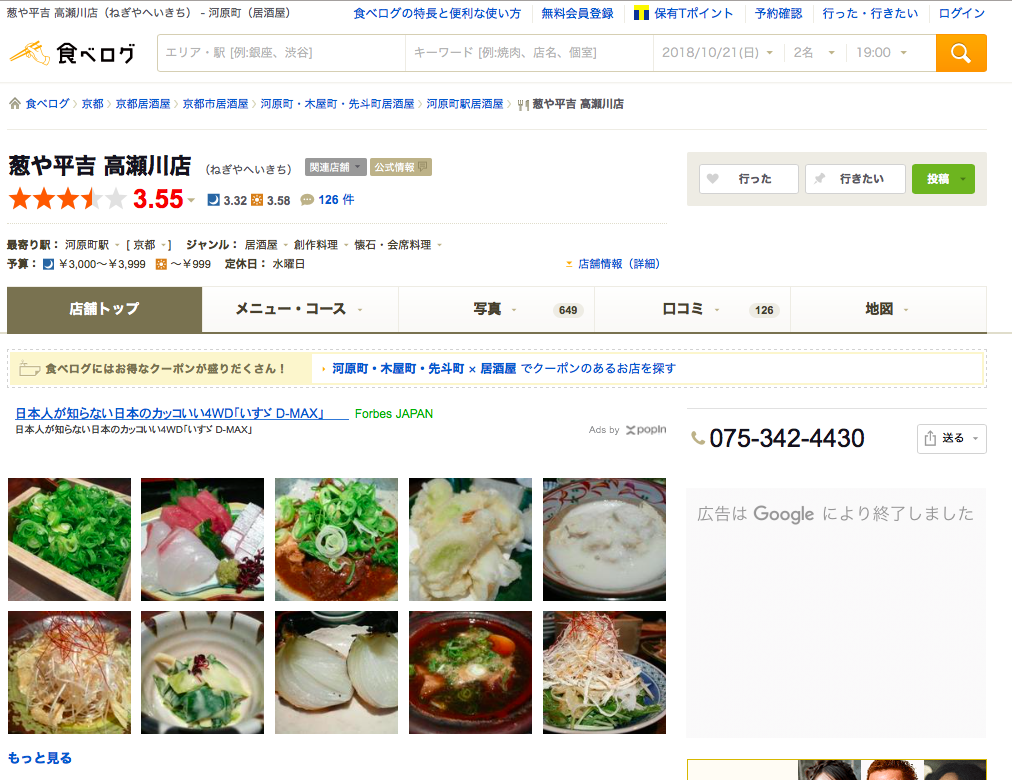
\includegraphics[clip,scale=0.25]{negiya.png}
\caption{葱や平吉の概要。なんか評価高い。カス。}
\label{negiya}
\end{figure}

もう一つは、(ポ)である。なんかやたらとネギを推す重症患者であり、そんなネギ好きの人たちにお勧めしたいのが「葱や平吉」である。

\begin{figure}[H]
\centering
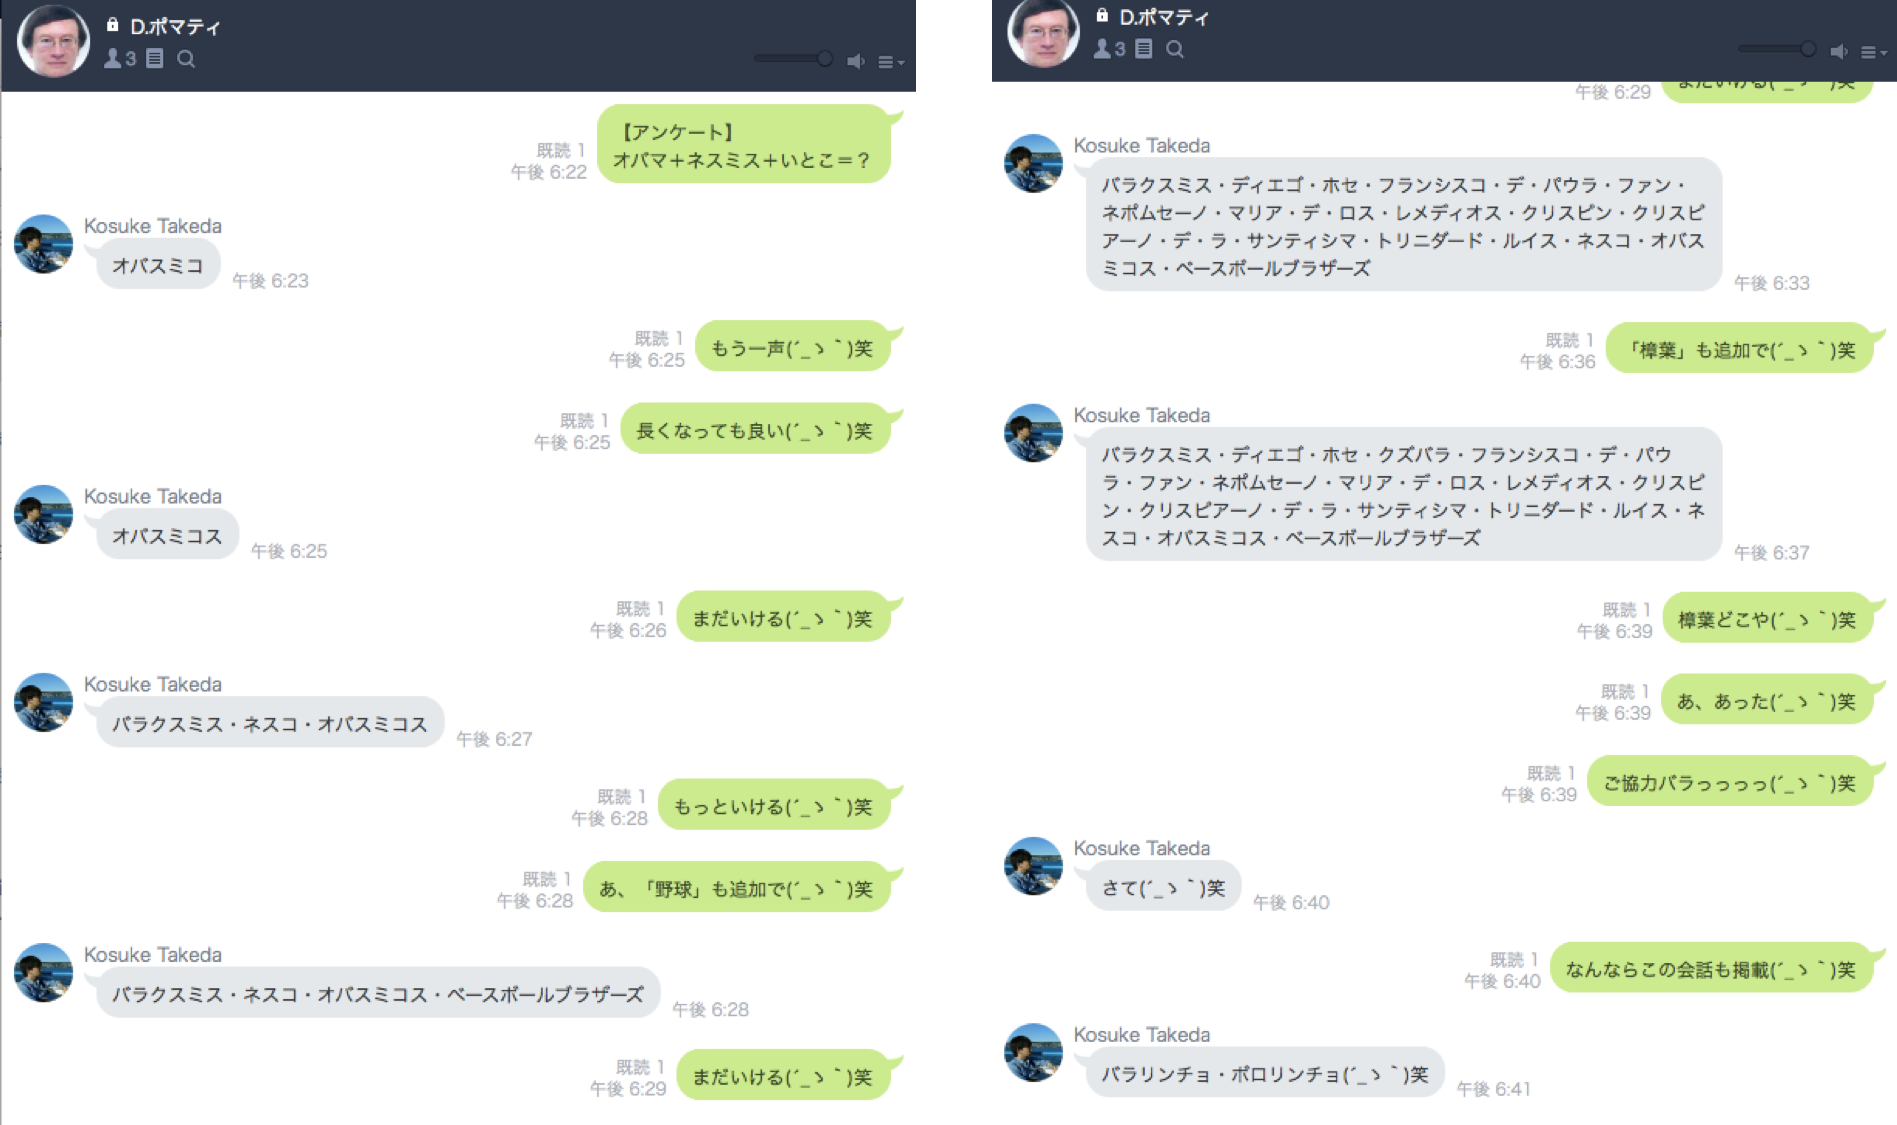
\includegraphics[clip,scale=0.3]{itoko.png}
\caption{いとこの生成過程。}
\label{itoko}
\end{figure}

\begin{figure}[H]
\centering
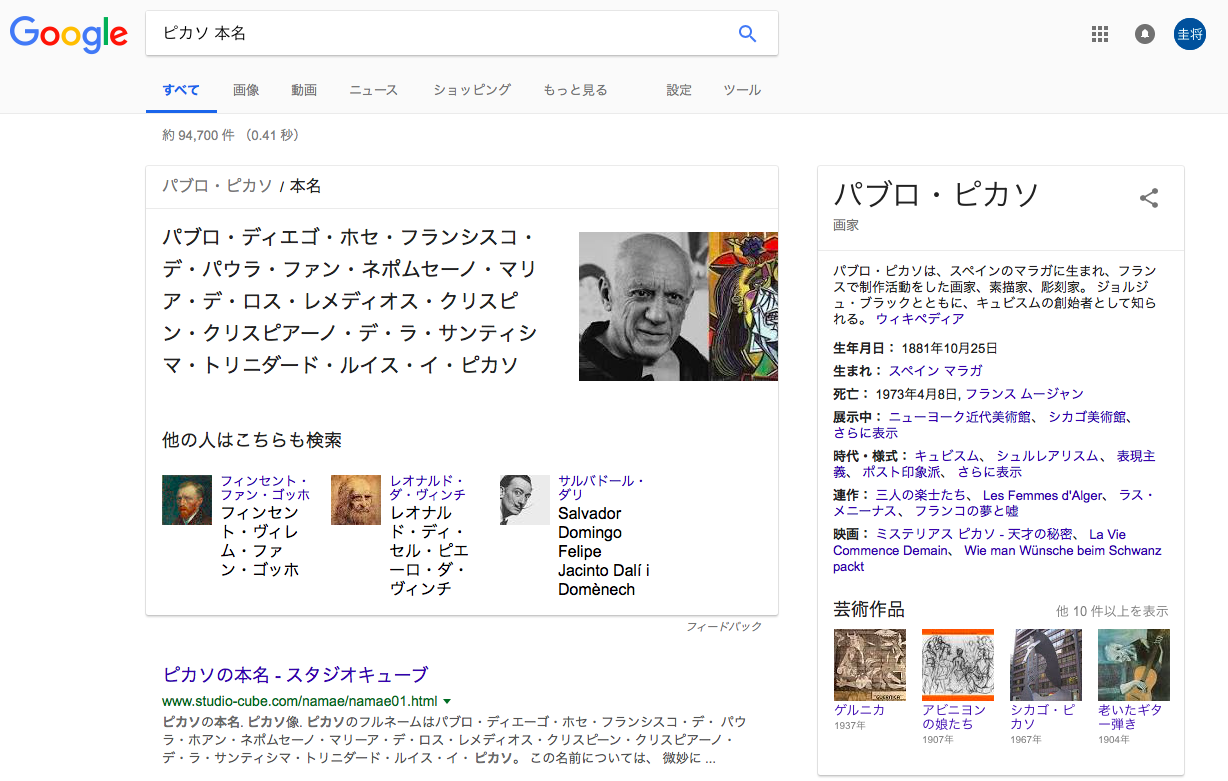
\includegraphics[clip,scale=0.25]{itoko2.png}
\caption{ヒント:ピカソ}
\label{itoko2}
\end{figure}

%==========================
\section{シャワログの口コミ}
%============================
宇宙で最も認知度のある口コミサイト「シャワログ」にて、葱や平吉の口コミが発掘されたので、ここで紹介する。

\begin{itemize}
\item カープカープ カープカープ(1945)さんの口コミ[携帯電話番号認証済] 30代後半・男性・広島県\\
京都の四条で、ランチをしようと探していると。\\
行列の出来ているお店発見!!!\\
京都の高島屋から歩いて5分程度の場所の小川沿いのお店です。\\
ネギがメインの珍しいお店です。\\

\item にのみや なな にのみや なな(177)さんの口コミ[携帯電話番号認証済]女性・京都府\\
個人的にはこちらのすぐ近くの中華屋さんに行きたかったのですが、あまりにも中華屋さんに行く回数が多すぎるとNGを食らってしまいました。\\
今後、中華屋さん行くときは一人になりそうです。(以下略)\\

\item 安倍太郎 安倍太郎(1122)さんの口コミ[携帯電話番号認証済]男性\\
1人でトロロ単品は嬉しくも危険な量!笑\\
此方のお店は紅虎餃子房で有名な際コーポレーションさんが運営するお店ですね。\\
昼時はいつでも行列が出来ており、一度は行って観たいと思っておりましたので\\
基本、並ぶのは嫌いなのですが行って参りました。(以下略)\\

\item カオリンゴ カオリンゴ(45)さんの口コミ[携帯電話番号認証済]
女性・東京都\\
雰囲気がいいです\\

最近、九条葱が美味しいお店に行ったのがきっかけで、他にも葱のお店があるかと知人がこちらを発見。\\
6人で行ったので色々な種類のお料理を注文しました。\\
特に美味しかったのは白葱サラダです(以下略)。\\
\end{itemize}

%=====================
\section{キックオフ}
%=====================
\label{hagehage}
そもそもMISUKE(以下ミスケ)とは、オガワマンの彼女である。オガワマンの会社の同期である彼女(みゆう)が「オガワマンの学生時代のエピソードを聞きたい」とか言いだしていた時代、どうしても研究室関連の話が同時多発してしまうという現象が観測されていた。そこで頻繁に生成されていた重症患者のfirst nameが「こうすけ」及び「ゆうすけ」、そしてオガワマンが「けいすけ」であったため、彼女の名前がミスケになってしまった。\\
ちなみにオアグァマンの学部時代の重症患者の一人のヒゲの本名は「だいすけ」であり、オガワマンの中学の親友であるハゲの本名も「ゆうすけ」である。\\

%======
\section{試合会場}
後に後世に語り継がれることになる伝説の試合会場は、静岡県裾野市の居酒屋「串特急」である(図\ref{kusitokkyuu})。本社がある地域自体がオガワマンが引くくらいの田舎で、まあまあの確率でこの会場が使用される。店員に「腕相撲が得意です!私に勝てばビール一杯無料!」とかイキってる兄ちゃんがいており、日中はトラックの運転手をしているため腕力ガチ勢である。オガワマンは両手を使って挑んだが、逆に体を支えることが不可能になり机の角が腹に刺さって死亡した(ほぼ実話)。\\


\begin{figure}[H]
\centering
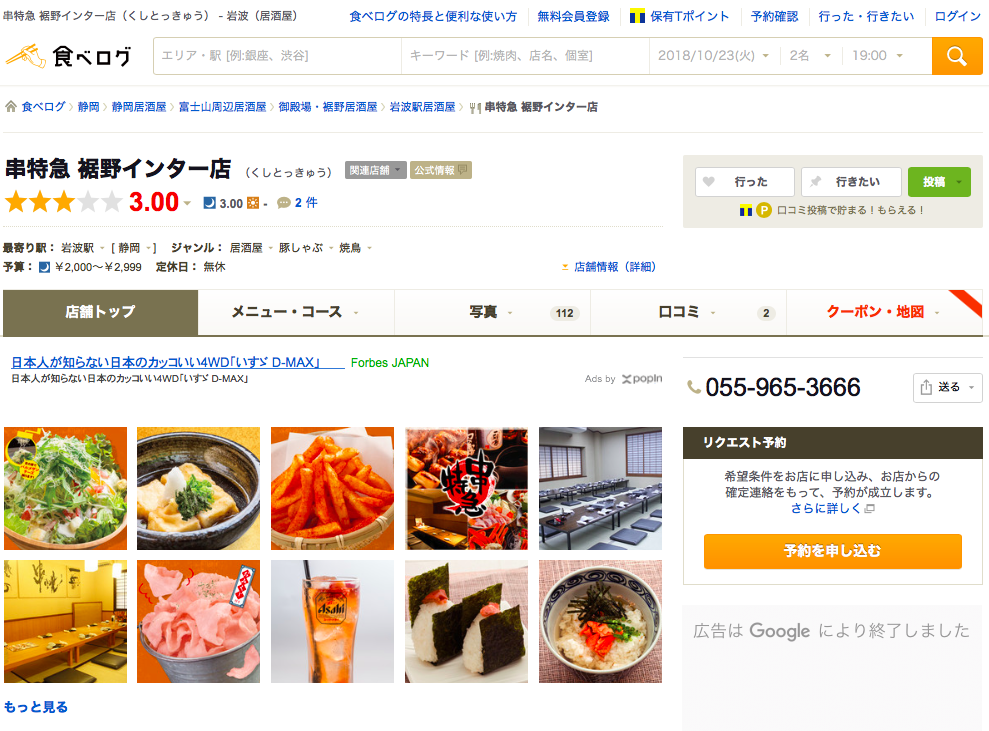
\includegraphics[clip,scale=0.25]{kusitokkyuu.png}
\caption{串特急の概要。なかなかの高評価。}
\label{kusitokkyuu}
\end{figure}

そもそもオガワマンが働いているオセチ工場株式会社(図\ref{oseti})では、入社後に二ヶ月間、静岡県での新入社員研修が存在する。その後1年間、全国各地の関連工場で実習を行う。つまり最終的にオセチになるのは1.5年後で、意味不明である。カス。

\begin{figure}[H]
\centering
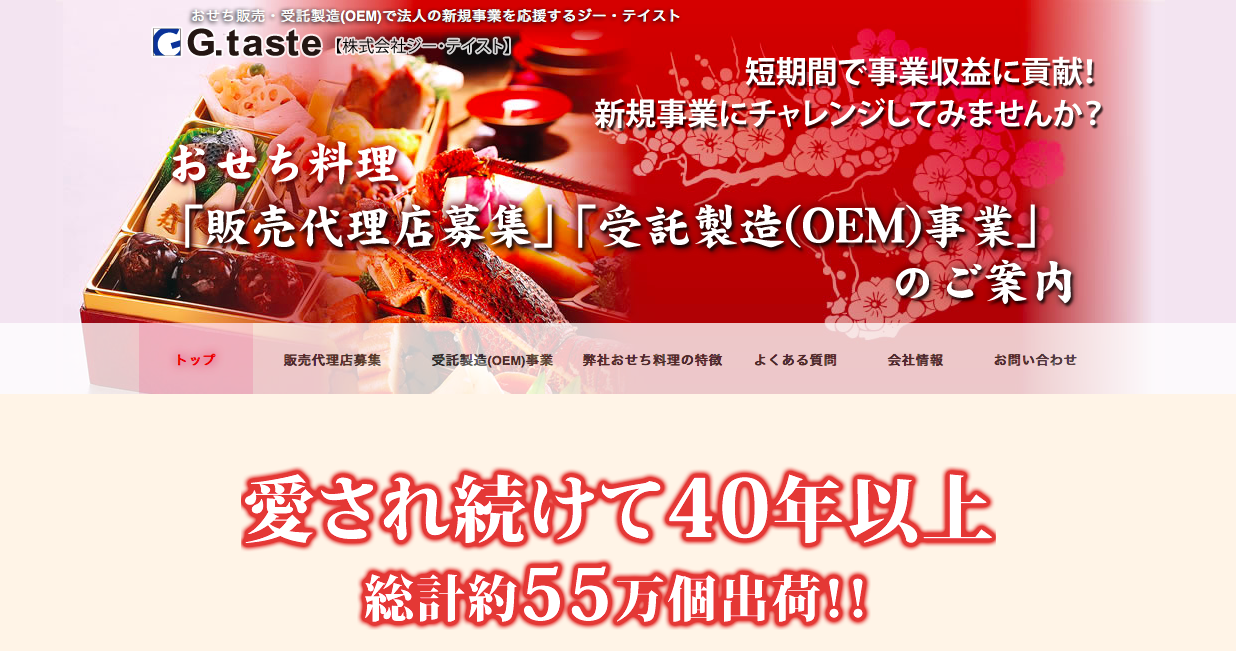
\includegraphics[clip,scale=0.2]{oseti.png}
\caption{オセチ工場株式会社。特にOEM(Osechi EnterteinMent)事業は年間生産量1億トン、世界人口の約0.827‰を顧客に持つと言っても過言。}
\label{oseti}
\end{figure}

%========
\section{キックオフの詳細}


その静岡県での新入社員研修が始まって一週間が経った週末に、さっそく新入社員の一部で飲み会を開こうということになった。人づてでその誘いが来たオガワマンであるが、正直せっかくの休日やし休みたいし飲み会とかダルいと思っていたが、なんか最初やし断るのもあれやな、みたいな感じで行くことになった。そこでは新入社員約100人のうち40人ほど参加しており、どいつもこいつもウンコやな、とか思いながら関西代表としてテンションぶちあげ大学院生をかましていたオガワマンであった。最初座った席のメンツが陰キャ臭かったため、とうとうオガワマンが濁流のように目まぐるしく変化する人々の飲み会座席ポジション変化第一弾をかまして辿り着いた集団の中にいたのが、ミスケである。奇しくも、オガワマンのシャツとミスケのブラウスが同じ色であったため、アバポンヌアブラサテである(図\ref{misuke1})。\\

\begin{figure}[H]
\centering
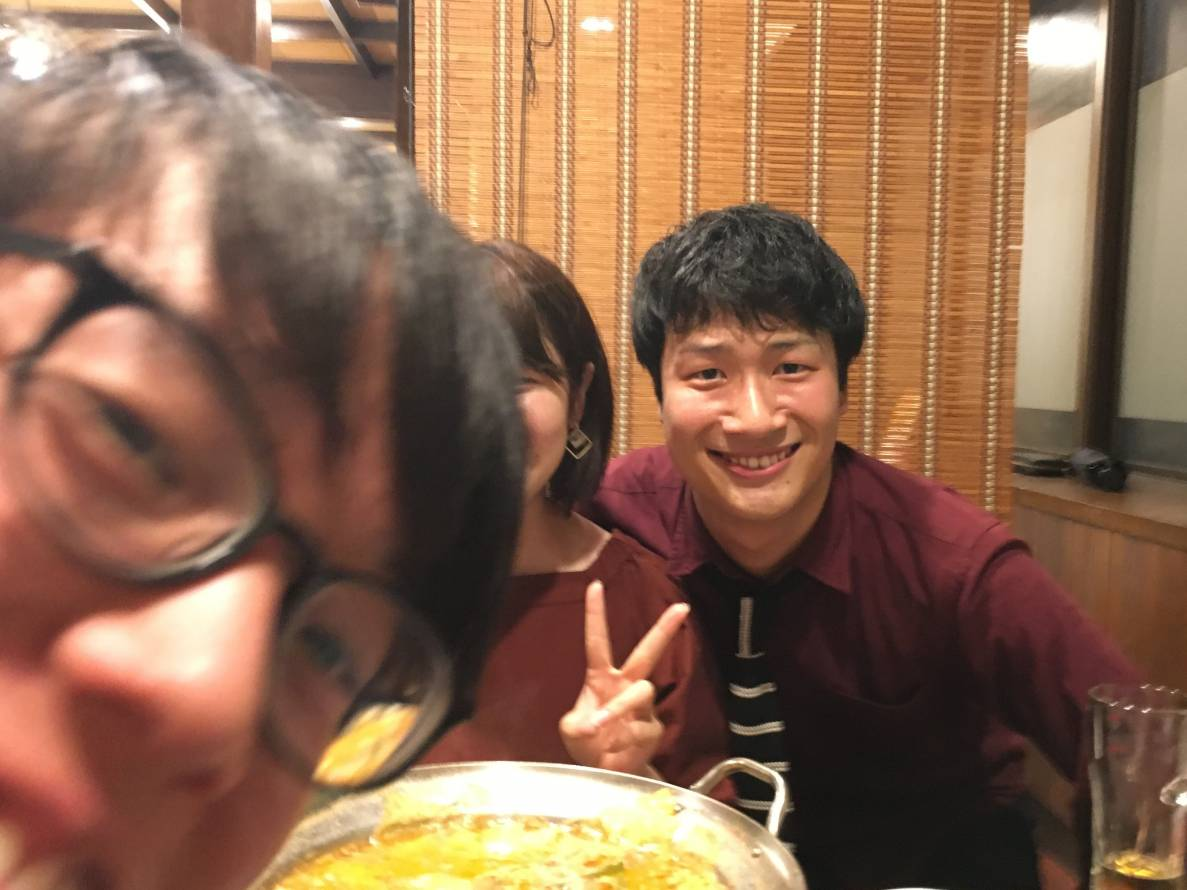
\includegraphics[clip,scale=0.18]{misuke1.jpg}
\caption{オガワマンとミスケが相対した瞬間。}
\label{misuke1}
\end{figure}



試合中はなんかまあ席を移動した時に目の前にあった唐揚げてきなやつとか鍋とかを適当に色々食べ、飲み物としては安定の最初だけビールと伝家の宝刀カシオレであった。その後、飲み会が終わりさっさと解散したが、周りにもはや店がないため、締めのラーメンという概念が消失するという「概念消失現象」が生じたのである。
ラーメンがどうとかそんなんどうでもよくて、この「概念消失現象」は太古の昔から人間どもが何億年もかけて解決に挑んではハゲ散らかして死滅していった難題である。\\
 しかし、この人類最大の困難に立ち向かった大御所重症患者がいた。概念は永久に不滅であります、こと、ミスタージャイアン・薔薇嶋薔薇男(100180)である。彼は、死に際、以下のようにtweetした。\\
 \\
\shadowbox{
\begin{tabular}{l}
概念が消失するということは、「概念が消失する」という概念が\\
生まれることにほか他ならない。
\end{tabular}}
 \\
\shadowbox{
\begin{tabular}{l}
概念が消失するということは、消失するという概念が消失すると\\
いうことである。
\end{tabular}}
 \\
\shadowbox{
\begin{tabular}{l}
結局、概念は不滅$\sf{ (´\_ゝ`)}$笑
\end{tabular}}
 \\
ばらっっっっっっっっっっっ$\sf{ (´\_ゝ`)}$笑

%======================
\section{コク把握}
%======================
ラーメンは、コクが命である。つまり、そのコクを把握したものこそが真の勝者である。\\
 伝説の試合会場での試合後、オガワマンとミスケは数々の共通の知人とのショッピングロケやカンファレンス、ジムトレーニング、ドラッグストア、目薬、パピコ、チョコなどのバチバチの殴り合いの末、来る某日、コクの把握に成功した。しかし、コクの把握の把握をしている人間はオガワマンとミスケ以外にはおらず、現在もその詳細な研究が進められており、2019年の新元号がカギを握ると言われている。またこの時、オガワマンとミスケは弊社とは別の会社の社宅の敷地内にたむろしていた。そもそも研修中やし、基本的に日中は仕事、定時で退勤後はジムに行くか飲みに行くか買い物に行くかしかすることがない。まあ個人的にも幾度となく会っていたわけだが、その日は曇りの夜やし暗いし寒いし、オガワマンに至ってはスウェットにチェックシャツという寝間着スタイルであったそうな。未だにミスケから「なぜあのような格好であったのか」と問い詰めてくることがあるという。ばらぼん。\\

%======================
\section{The name somebody goes by...}
%======================
\begin{figure}[H]
\centering
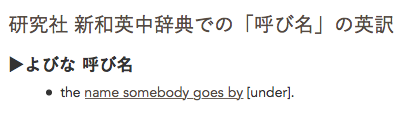
\includegraphics[clip,scale=0.5]{weblio.png}
\caption{Weblio久々に使った}
\label{weblio}
\end{figure}



まあカップルの情報としてお互いの呼び名が気になるってのはわからんでもないが、残念ながらそこまで面白い展開はない$\sf{ (´\_ゝ`)}$笑\\
 とは言っても一応掲載する程度の語るべくいかにその努力の痕跡を残す。図\ref{yobina}はその変遷を表した呼び名生成過程のアイーンマン図である\footnotetext{この概念は、便座学会の大御所、志村便によって提唱されたと云われている。志村便はかの有名なベン図も手がけたことでおなじみ。ベン図を手がけるという概念。}。そもそもお互いが仲良くなるまではOgawa-kun, Abe-sanとなる。しかし、オガワマンの場合、研修中に共同生活していた男達にKeisukeと呼ばれていたので初対面のときからKeisukeと呼ばれていた。一方ミスケの場合、地元が田舎であるがゆえ、周りがAbeだらけなのである。そのため、基本的には下の名前で呼ばれることが多く、むしろ初対面の時から「苗字で呼ばれたくない」との趣旨の発言をしていたとのこと。したがって初対面の時からMiyuuであった。付き合い始めてからも基本的にKeisuke, Miyuuであったが、時折、Kei-uen・Miyu interactionを観測する事があるという。しかしまだこの現象を理論的に証明できる天才重症患者が世界中の病院にはいないため、より詳細な研究がもとめられると言っても過言。\\
 \\
 
\begin{figure}[H]
\centering

\includegraphics[clip,scale=0.6]{yobina.png}
\caption{オガワマンとミスケの互いの呼び名の変遷アイーンマン図。}
\label{yobina}
\end{figure}

%======================
\section{結論}
%======================
2018年現在、挙式の予定は決まっていない。真面目な話、オアグァマンとミスケは同じ会社の同期同士であり、勤務地が静岡と広島であるため、なかなかタイミングを決めるのが難しいのである。しかし、普段から結婚についての話題は頻繁に出ているため、まあ挙式の予定としては、近い将来する事になるでしょう。また、挙式のスタイルはナチュラルテイストな感じがいいらしいです。お互いの実家が宮城&京都、大学が千葉&神戸と全国規模であるため、誰を招待して(これが結構難しい)、どの場所で行うかによって挙式の規模や予算などが変わってくる。よって挙式については今後より詳細な研究がもとめられる。日にちは正味、三連休の中日とかの方がよくね?とは思うけど。研究室の奴らとかどうなんやろ、呼んだら来てくれるんかな?ありがたいけど(笑)\\
 参考画像としてミスケが提示してきたものを図\ref{zekusi}に示す。\\

\begin{figure}[H]
\centering
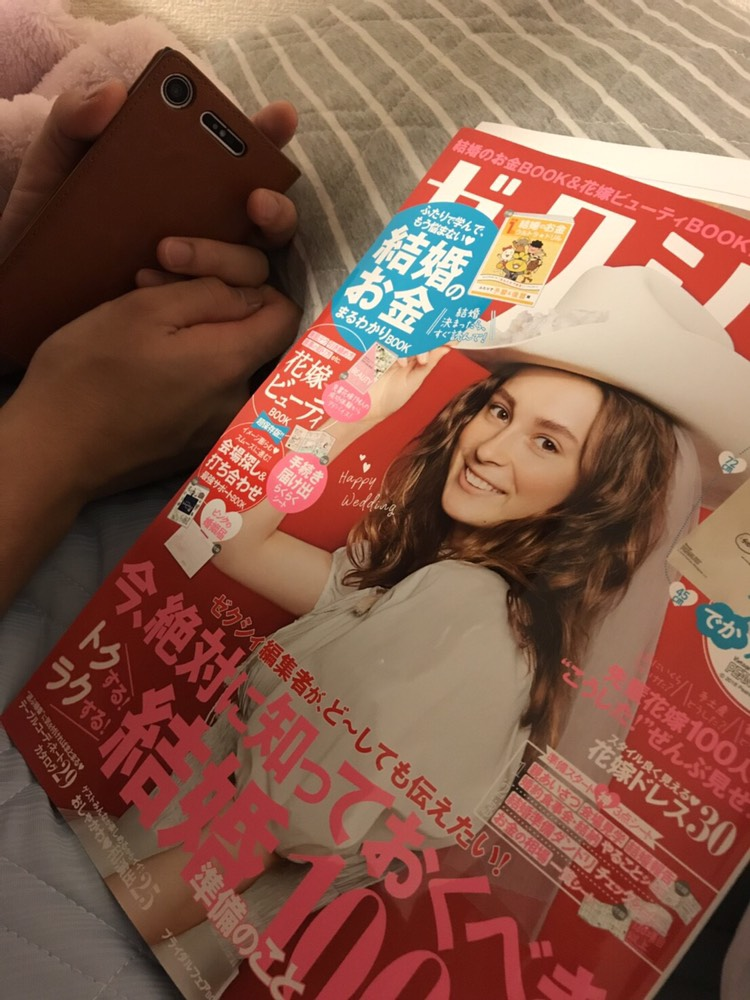
\includegraphics[clip,scale=0.3]{zekusi.jpg}
\caption{ゼクシイ。なんかミスケがほしいグッズが付録にあった模様。まあちょくちょく買ってるけど$\sf{ (´\_ゝ`)}$}
\label{zekusi}
\end{figure}





%%%%%%%%%%%%%%%%%%%%%%%%%%%%%
